% Standalone insertion fragment. Add \usepackage{graphicx} to the preamble.
% Keep false_detection_comparison.pdf beside the manuscript, or adjust the path.
% No main manuscript file is modified by this experiment.
\begin{figure*}[t]
  \centering
  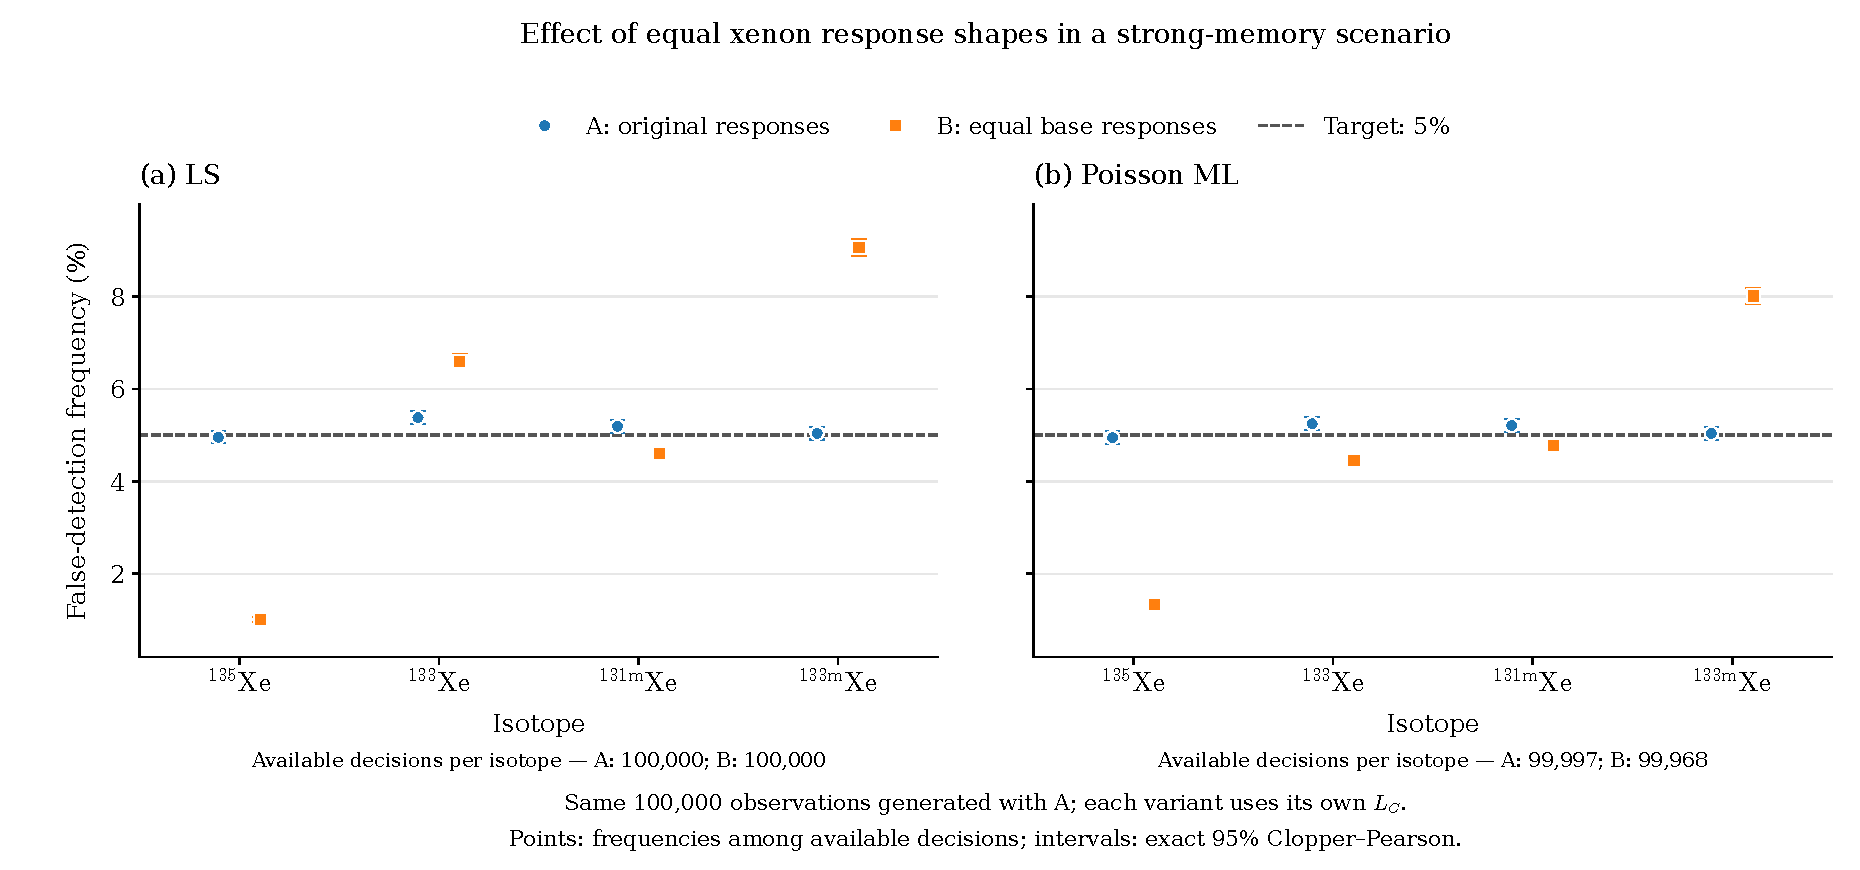
\includegraphics[width=\textwidth]{false_detection_comparison.pdf}
  \caption{False-detection frequencies for (a) weighted least squares and
  (b) unconstrained Poisson maximum likelihood in the strong-memory scenario.
  The same 100\,000 observation vectors were generated with the original
  response model A. Model B uses the fresh-sample base response shapes for
  the four xenon components in gas memory; decay, daughter ingrowth,
  measurement times, and all other conditions are retained.
  Each variant uses its own auxiliary nonnegative fit and critical level
  $L_C$, without threshold rescaling. Points and error bars denote empirical
  frequencies among available decisions and exact marginal 95\% Clopper--Pearson
  intervals. The dashed line marks the 5\% target for each isotope.}
  \label{fig:xemat-equal-memory-responses}
\end{figure*}
